\scanpage{9}

% ll. 1–5
\mspage{\textcircled{7}}
$\unsure{\zeta|z|\xi}=\eta$, d'où l'injectivité. Montrons que $\Gamma$ est stable par les éléments de $N_u=\operatorname{Ker}(\Psi\xrightarrow{\mathrm{pr}_1}V)$ (donc aussi par $N_v$ et $N_w$) --- il s'ensuivra qu'il est stable par $\Psi\underset{\unsure{?|\gamma}}{=}N_u+N_v$, donc (étant de cardinal $16=\operatorname{card}\Psi$) c'est un torseur sous $\Psi$. \unsure{Cela|Ceci} équivaut au

% ll. 6–9
\uline{Corollaire} Soit $x\in E(u)^*$, $s\in E(v)^*$, $\zeta\in E(w)^*$ formant triangle. \deleted{Alors} Soit \deleted{\unsure{$q$}} $t\in E(v)^*$ \inserted{$t\ne s$} non lié à $s$, et lié à $\zeta$ (il y en a trois), et soit $\eta$ l'élmt de $E(w)^*$ distinct de $\zeta$ lié à $s,t$ (lemme 4). Alors

% l. 10
\[
\deleted{\unsure{\varphi}}(\pi_u(x),\pi_{\unsure{u|v}}(t),\pi_{\unsure{u|w}}(\eta))\in\operatorname{Im}(\Gamma\longrightarrow P_u\times P_v\times P_w),
\]

% ll. 11–13
\deleted{i.e. $\{x,\eta,t\}$ est un triangle, ou un} \deleted{Alors} plus précisément $(x,\sigma t,\sigma\eta)$ est un triangle.

% left of corollary
\figure{\begin{tikzpicture}[scale=.86]
\draw (0,1) node[above left] {$v$} -- (1.2,.74) node[right] {$w$} -- (.16,0) node[below] {$u$} -- cycle;
\draw (.32,.70)--(.61,.92);
\node at (-.12,2.25) {$\zeta$}; \node at (.36,2.25) {$\eta$};
\node at (2.45,.80) {$\unsure{t}$}; \node at (2.52,.47) {$s$}; \node at (-.2,-.90) {$x$};
\end{tikzpicture}}

% ll. 14–18
\uline{Dém} Comme $x$ est lié à $s$ et $\zeta$, liés resp. à $\eta$ et $t$, il ne peut être lié à $t$ ni $\eta$, donc il est lié à $\sigma t$ et $\sigma\eta$, qui sont liés entre eux (\deleted{qui} puisque $t$ et $\eta$ le sont) cqfd.

% left of demonstration
\figure{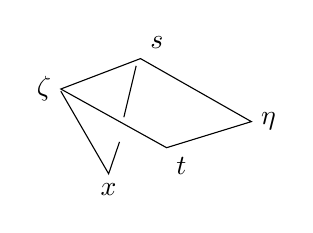
\begin{tikzpicture}[scale=.92]
\draw (0,.7) node[left] {$\zeta$} -- (1.10,1.12) node[above right] {$s$} -- (2.63,.25) node[right] {$\eta$} -- (1.46,-.11) node[below right] {$t$} -- cycle;
\draw (0,.67)--(.66,-.47) node[below] {$x$} -- (.81,-.03) (1.04,1.02)--(.87,.31);
\end{tikzpicture}}

% ll. 19–25
\uline{NB} La donnée de $V$ et du torseur $\Gamma$ sous $\Psi(\unsure{W|V})$ permet de réconstituer $P_u,P_v,P_w$ et la notion de ``triangles'' dans $P_u\times P_v\times P_w$. Il faut encore réconstituer les rev. à 2 feuillets $E(u)^*\inserted{=\widetilde P_u},E(v)^*\inserted{=\widetilde P_v},E(w)^*\inserted{=\widetilde P_w}$ de $P_u,P_v,P_w$, et le \unsure{revêmt|revêment|revêtement} à 2 feuillets $\unsure{\widetilde{\mathscr T}|\widetilde\Gamma}$, et les liens $\widetilde\Gamma\mathbin{-}\widetilde P_u$ etc sur $\Gamma\to P_u$ etc. $\big]$

\noindent ---
% archive sheet number: 8
